\documentclass[11pt,compress,t,notes=noshow, xcolor=table]{beamer}
\usepackage[]{graphicx}\usepackage[]{color}
% maxwidth is the original width if it is less than linewidth
% otherwise use linewidth (to make sure the graphics do not exceed the margin)
\makeatletter
\def\maxwidth{ %
  \ifdim\Gin@nat@width>\linewidth
    \linewidth
  \else
    \Gin@nat@width
  \fi
}
\makeatother

\newcommand{\citebutton}[2]{%
\beamergotobutton{\href{#2}{#1}}%
}

\newcommand{\blu}[1]{\textcolor{blue}{#1}}
\newcommand{\org}[1]{\textcolor{orange}{#1}}
\newcommand{\ques}{\textbf{\textcolor{red}{Question:  }}}
\newcommand{\questionssofar}{\begin{frame}\frametitle{Any questions?}\end{frame}}

\newcommand\warning{%
 \makebox[1.4em][c]{%
 \makebox[0pt][c]{\raisebox{.1em}{\scriptsize!}}%
 \makebox[0pt][c]{\color{red}\normalsize$\bigtriangleup$}}}%

\definecolor{fgcolor}{rgb}{0.345, 0.345, 0.345}
\newcommand{\hlnum}[1]{\textcolor[rgb]{0.686,0.059,0.569}{#1}}%
\newcommand{\hlstr}[1]{\textcolor[rgb]{0.192,0.494,0.8}{#1}}%
\newcommand{\hlcom}[1]{\textcolor[rgb]{0.678,0.584,0.686}{\textit{#1}}}%
\newcommand{\hlopt}[1]{\textcolor[rgb]{0,0,0}{#1}}%
\newcommand{\hlstd}[1]{\textcolor[rgb]{0.345,0.345,0.345}{#1}}%
\newcommand{\hlkwa}[1]{\textcolor[rgb]{0.161,0.373,0.58}{\textbf{#1}}}%
\newcommand{\hlkwb}[1]{\textcolor[rgb]{0.69,0.353,0.396}{#1}}%
\newcommand{\hlkwc}[1]{\textcolor[rgb]{0.333,0.667,0.333}{#1}}%
\newcommand{\hlkwd}[1]{\textcolor[rgb]{0.737,0.353,0.396}{\textbf{#1}}}%
\let\hlipl\hlkwb

\usepackage{framed}
\makeatletter
\newenvironment{kframe}{%
 \def\at@end@of@kframe{}%
 \ifinner\ifhmode%
  \def\at@end@of@kframe{\end{minipage}}%
  \begin{minipage}{\columnwidth}%
 \fi\fi%
 \def\FrameCommand##1{\hskip\@totalleftmargin \hskip-\fboxsep
 \colorbox{shadecolor}{##1}\hskip-\fboxsep
     % There is no \\@totalrightmargin, so:
     \hskip-\linewidth \hskip-\@totalleftmargin \hskip\columnwidth}%
 \MakeFramed {\advance\hsize-\width
   \@totalleftmargin\z@ \linewidth\hsize
   \@setminipage}}%
 {\par\unskip\endMakeFramed%
 \at@end@of@kframe}
\makeatother

\definecolor{shadecolor}{rgb}{.97, .97, .97}
\definecolor{messagecolor}{rgb}{0, 0, 0}
\definecolor{warningcolor}{rgb}{1, 0, 1}
\definecolor{errorcolor}{rgb}{1, 0, 0}
\newenvironment{knitrout}{}{} % an empty environment to be redefined in TeX

\usepackage{alltt}
\newcommand{\SweaveOpts}[1]{}  % do not interfere with LaTeX
\newcommand{\SweaveInput}[1]{} % because they are not real TeX commands
\newcommand{\Sexpr}[1]{}       % will only be parsed by R
\newcommand{\xmark}{\ding{55}}%


\usepackage[english]{babel}
\usepackage[utf8]{inputenc}

\usepackage{dsfont}
\usepackage{verbatim}
\usepackage{amsmath}
\usepackage{amsfonts}
\usepackage{amssymb}
\usepackage{bm}
\usepackage{csquotes}
\usepackage{multirow}
\usepackage{longtable}
\usepackage{booktabs}
\usepackage{enumerate}
\usepackage[absolute,overlay]{textpos}
\usepackage{psfrag}
\usepackage{algorithm}
\usepackage{algpseudocode}
\usepackage{eqnarray}
\usepackage{arydshln}
\usepackage{tabularx}
\usepackage{placeins}
\usepackage{tikz}
\usepackage{setspace}
\usepackage{colortbl}
\usepackage{mathtools}
\usepackage{wrapfig}
\usepackage{bm}
\usepackage{amsmath}
\usepackage{pifont}

\usetikzlibrary{shapes.multipart,shapes,arrows,automata,positioning,calc,chains,trees, shadows}
\tikzset{
  %Define standard arrow tip
  >=stealth',
  %Define style for boxes
  punkt/.style={
    rectangle,
    rounded corners,
    draw=black, very thick,
    text width=6.5em,
    minimum height=2em,
    text centered},
  % Define arrow style
  pil/.style={
    ->,
    thick,
    shorten <=2pt,
    shorten >=2pt,}
}

\tikzstyle{vec}=[draw, rectangle, fill = white, minimum width=5mm, minimum height=1cm, inner sep = 2pt]

\usepackage{subfig}

% Defines macros and environments
\usepackage{../../style/lmu-lecture}


\let\code=\texttt
\let\proglang=\textsf

\setkeys{Gin}{width=0.9\textwidth}

\setbeamertemplate{frametitle}{\expandafter\uppercase\expandafter\insertframetitle}

\usepackage{bbm}
% basic latex stuff
\newcommand{\pkg}[1]{{\fontseries{b}\selectfont #1}} %fontstyle for R packages
\newcommand{\lz}{\vspace{0.5cm}} %vertical space
\newcommand{\dlz}{\vspace{1cm}} %double vertical space
\newcommand{\oneliner}[1] % Oneliner for important statements
{\begin{block}{}\begin{center}\begin{Large}#1\end{Large}\end{center}\end{block}}


%new environments
\newenvironment{vbframe}  %frame with breaks and verbatim
{
 \begin{frame}[containsverbatim,allowframebreaks]
}
{
\end{frame}
}

\newenvironment{vframe}  %frame with verbatim without breaks (to avoid numbering one slided frames)
{
 \begin{frame}[containsverbatim]
}
{
\end{frame}
}

\newenvironment{blocki}[1]   % itemize block
{
 \begin{block}{#1}\begin{itemize}
}
{
\end{itemize}\end{block}
}

\newenvironment{fragileframe}[2]{  %fragile frame with framebreaks
\begin{frame}[allowframebreaks, fragile, environment = fragileframe]
\frametitle{#1}
#2}
{\end{frame}}


\newcommand{\myframe}[2]{  %short for frame with framebreaks
\begin{frame}[allowframebreaks]
\frametitle{#1}
#2
\end{frame}}

\newcommand{\remark}[1]{
  \textbf{Remark:} #1
}


\newenvironment{deleteframe}
{
\begingroup
\usebackgroundtemplate{
\includegraphics[width=\paperwidth,height=\paperheight]{../style/color/red.png}}
 \begin{frame}
}
{
\end{frame}
\endgroup
}
\newenvironment{simplifyframe}
{
\begingroup
\usebackgroundtemplate{
\includegraphics[width=\paperwidth,height=\paperheight]{../style/color/yellow.png}}
 \begin{frame}
}
{
\end{frame}
\endgroup
}\newenvironment{draftframe}
{
\begingroup
\usebackgroundtemplate{
\includegraphics[width=\paperwidth,height=\paperheight]{../style/color/green.jpg}}
 \begin{frame}
}
{
\end{frame}
\endgroup
}
% https://tex.stackexchange.com/a/261480: textcolor that works in mathmode
\makeatletter
\renewcommand*{\@textcolor}[3]{%
  \protect\leavevmode
  \begingroup
    \color#1{#2}#3%
  \endgroup
}
\makeatother





\input{../../latex-math/basic-math.tex}
\input{../../latex-math/basic-ml.tex}

\usepackage{tikz}
\usetikzlibrary{positioning}


\newcommand{\titlefigure}{}
\newcommand{\learninggoals}{
\item Understand which components of the Transformer contribute to the parameter count
\item Learn how to calculate the total number of the model parameters}

\title{Transformer}
% \author{}
\institute{\href{https://slds-lmu.github.io/lecture_dl4nlp/}{slds-lmu.github.io/lecture\_dl4nlp}}
\date{}

\begin{document}
\lecturechapter{Transformer Parameter Count}
\lecture{Deep Learning for NLP}
% ------------------------------------------------------------------------------

\begin{frame}{Why do we care about the Parameter Count?}
\begin{itemize}
    \item Being able to derive the parameter count of a model requires good knowledge of the math behind the model architecture
    \item So by deriving the parameter count we learn how the model works under the hood
    \item Since models just stack various buidling blocks on top of eachother, we can reuse the derived parameter count for all sorts of models
    \item We get an idea about how the parameters scale with increasing model size
\end{itemize}
\end{frame}

% ------------------------------------------------------------------------------

\begin{frame}{Overview over Parameter Sources}
\vfill
\begin{minipage}[c]{.49\textwidth}
    \vfill
    \begin{figure}
		\centering
		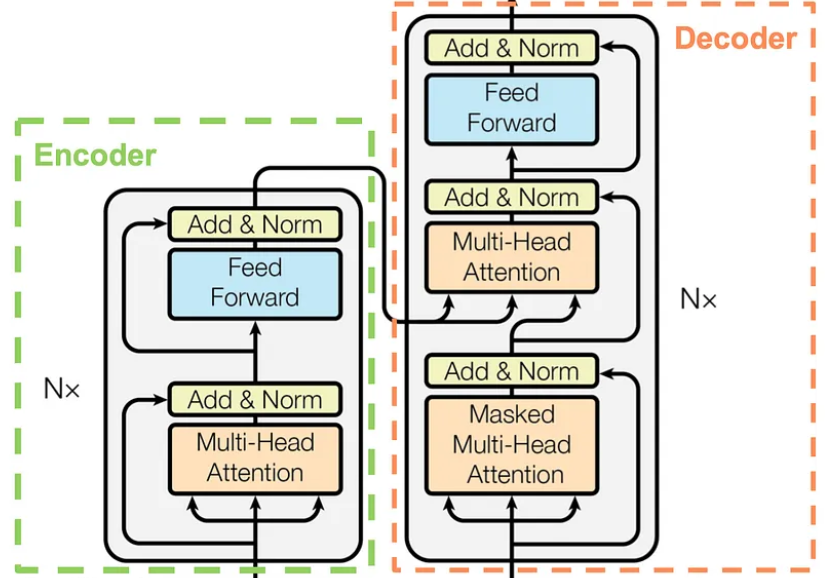
\includegraphics[]{chapters/chapter03/figure/enc_dec.png}
	\end{figure}
    \vfill
\end{minipage}
\hfill
\begin{minipage}[c]{.49\textwidth}
    \hfill
    \begin{itemize}
        \item \textbf{Encoder}
        \begin{itemize}
            \item Multi-Head Attention
            \item 2x Layernorm
            \item Feed Forward Network
        \end{itemize}
        \item \textbf{Decoder}
        \begin{itemize}
            \item 2x Multi-Head Attention
            \item 3x Layernorm
            \item Feed Forward Network
        \end{itemize}
    \end{itemize}
\end{minipage}
\vfill
\textit{So all we have to do is to derive the parameter count of each of those components and then sum them up!} \citebutton{Vaswani et al., 2017}{https://arxiv.org/abs/1706.03762}

\end{frame}

%-------------------------------------------------------------------------------

\begin{frame}{Multi Head Attention (1)}

\begin{minipage}[c]{.44\textwidth}
    \vfill
    \begin{figure}
        \centering
        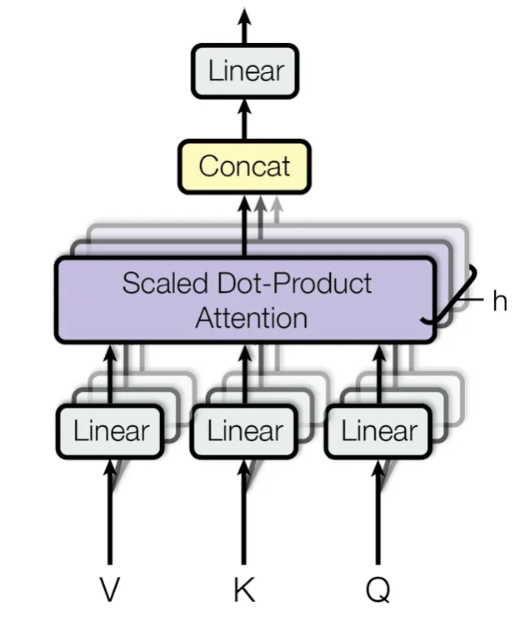
\includegraphics{chapters/chapter03/figure/mha.png}
        \label{fig:enter-label}
    \end{figure}
    \vfill
\end{minipage}
\hfill
\begin{minipage}[c]{.54\textwidth}
    \begin{itemize}
        \item The input token embeddings have shape $d_{model}$ (embedding dimension)
        \item Project input embeddings into Query, Keys and Values with matrices $\boldsymbol{W_Q}$, $\boldsymbol{W_K}$, $\boldsymbol{W_V}$ for each head (so we have $n_{head}$ ($h$ in the image) of each Matrix)
        \item Project concatenated output of the Scaled Dot-Product Attention back to $d_{model}$ with $\boldsymbol{W_O}$
    \end{itemize}
\end{minipage}
\vfill
\textit{To get to the total parameter count we simply have to calculate the number of parameters in all of those Matrices! (for now we also include the bias terms of the linear projections)}

    
\end{frame}

%-------------------------------------------------------------------------------

\begin{frame}{Multi Head Attention (2)}

\begin{itemize}
    \item \textbf{Project Input Sequence into Query, Key and Value:}
        \begin{itemize}
            \item Input shape: $seq\_len\times d_{model}$ ($seq\_len$ is the number of tokens, where each has the embedding dimension of $d_{model}$)
            \item For MHA we project $d_{model}$ to $d_{qkv}$, with $d_{qkv} = d_{model}/n_{head}$ \item We split up $d_{model}$ into $n_{head}$ heads and need $\boldsymbol{W_Q}$, $\boldsymbol{W_K}$, $\boldsymbol{W_V}$ for each head
            \item Each Matrix has shape $d_{model} \times d_{qkv}$
        \end{itemize}
    \vfill
    \item \textbf{Project concatenated output to the MHA output:}
        \begin{itemize}
            \item We concatenate the $n_{head}$ outputs, where each has shape $d_{qkv}$ and end up with a shape of $d_{model}$ again
            \item We then project $d_{model}$ to $d_{model}$ with $\boldsymbol{W_O}$
            \item $\boldsymbol{W_O}$ thus has a shape of $d_{model} \times d_{model}$
        \end{itemize}
\end{itemize}
    
\end{frame}

%-------------------------------------------------------------------------------

\begin{frame}{Multi Head Attention (3)}

\textit{Now we put both parts together:}

$$
\begin{aligned}
N_{attention} &= \underbrace{(d_{model} \times d_{model} + d_{model})}_{W_O} \\
&\quad + \underbrace{(d_{model} \times d_{qkv} + d_{qkv})}_{W_{Q,K,V}} \times \overbrace{n_{heads} \times 3}^{\text{3 matrices for each head}} \\
&= (d_{model} \times d_{model} + d_{model}) + (d_{model} \times d_{model} + d_{model}) \times 3 \\
&= \underbrace{(d_{model}^2 + d_{model}) \times 4}_{\text{The exact formula}} \\
&\approx \underbrace{4 \cdot d_{model}^2}_{\text{Approximation}}
\end{aligned}
$$

\end{frame}


%-------------------------------------------------------------------------------

\begin{frame}{Feed Forward Network}

\begin{minipage}[c]{.44\textwidth}
    \vfill
    \begin{figure}
        \centering
        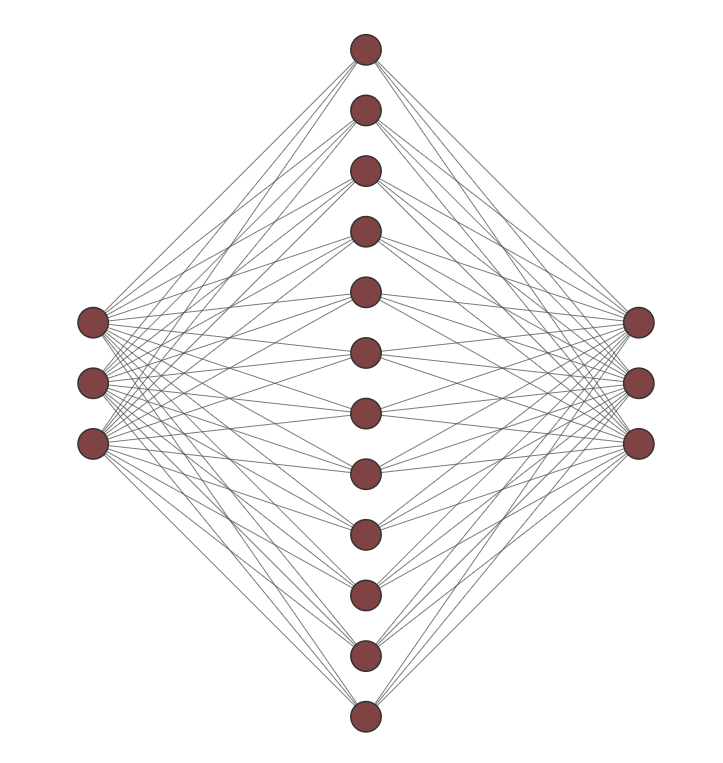
\includegraphics{chapters/chapter03/figure/ffn.png}
        \label{fig:enter-label}
    \end{figure}
    \vfill
\end{minipage}
\hfill
\begin{minipage}[c]{.54\textwidth}
    \begin{itemize}
        \item The FFN of the Transformer uses two fully connected layers
        \item Input and output size is both $d_{model}$
        \item The hidden layer size is $4 \times d_{model}$ (\textit{This is a decision by the authors of the paper!)}
        \item Our weight matrices $W_1$ and $W_2$ therefore have shape $d_{model} \times 4\cdot d_{model}$ and $4\cdot d_{model} \times d_{model}$ respectively
    \end{itemize}
\end{minipage}

$$
\begin{aligned}
N_{FFN} &= (d_{model} \times 4\cdot d_{model} +4\cdot d_{model}) + (4\cdot d_{model} \times d_{model} + d_{model}) \\
&= 8\cdot d_{model}^2 + 5\cdot d_{model} \\
&\approx 8\cdot d_{model}^2    
\end{aligned}
$$  

\end{frame}

%-------------------------------------------------------------------------------

\begin{frame}{Layer Norm (1)}

\begin{figure}
    \centering
    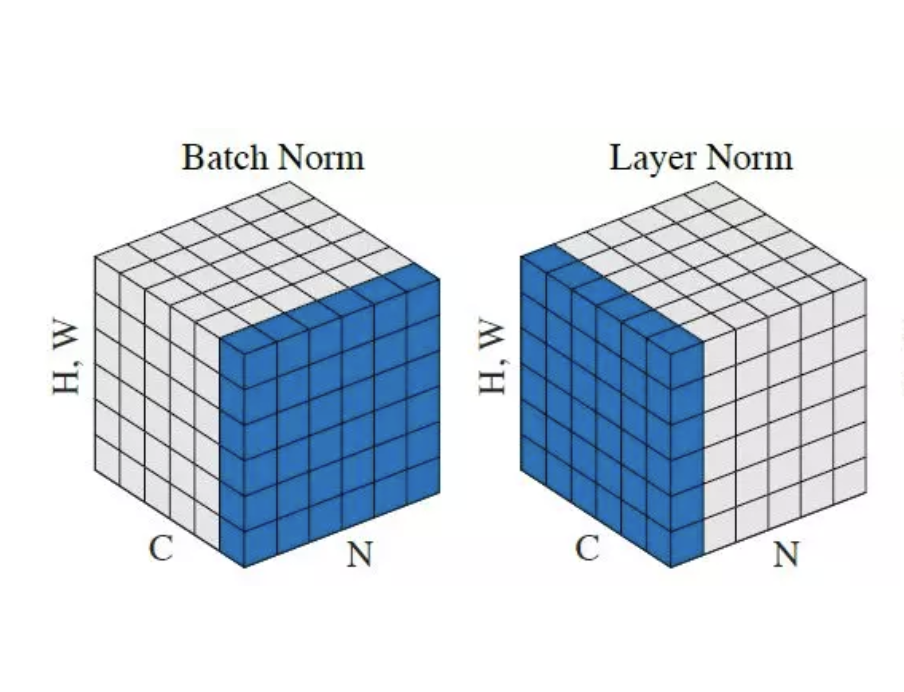
\includegraphics[width=7cm]{chapters/chapter03/figure/layernorm.png}    \label{fig:Layer Norm-label}
\end{figure}

\textit{Instead of calculating mean and standard deviation across the batch we do that across the layer!} \citebutton{Layer Normalization}{https://paperswithcode.com/method/layer-normalization}
    
\end{frame}

%-------------------------------------------------------------------------------

\begin{frame}{Layer Norm (2)}

\begin{itemize}
    \item We estimate $\mu$ and $\sigma$ for each layer (\textit{H denotes the number of hidden neurons in a layer}):
\end{itemize}
$$\mu = \frac{1}{N} \sum^{H}_{i=1}a_{i}$$
$$\sigma = \sqrt{\frac{1}{N} \sum^{H}_{i=1}{(a_{i}-\mu})^2}$$

\begin{itemize}
    \item For rescaling the normalizations we need a $\beta$ and $\gamma$ parameter for each neuron in the layer
    \item Since our layer has $d_{model}$ neurons we need $2\cdot d_{model}$ parameters for the Layer Norm operations
\end{itemize}

$$N_{Layernorm} = 2\cdot d_{model}$$
    
\end{frame}
%-------------------------------------------------------------------------------

\begin{frame}{Exact Parameter Count}
\textit{All we have to do now is to sum up the Parameter counts of each component for both the Encoder and Decoder!}

\begin{aligned}
$$
N_{Encoder} &= 1\cdot N_{attention} + 1\cdot N_{FFN} + 2\cdot N_{Layernorm} \\
&= 4\cdot(d_{model}^2 + d_{model}) + 8\cdot d_{model}^2 + 5\cdot d_{model} + 2\cdot(2\cdot d_{model}) \\
&= 12\cdot d_{model}^2 + 13 \cdot d_{model}
$$
\end{aligned}

\hspace{}

\begin{aligned}
$$
N_{Decoder} &= 2\cdot N_{attention} + 1\cdot N_{FFN} + 3\cdot N_{Layernorm}\\
&= 2\cdot 4\cdot (d_{model}^2 + d_{model}) + 8\cdot d_{model}^2 + 5\cdot d_{model} + 3\cdot (2\cdot d_{model}) \\
&= 16\cdot d_{model}^2 + 19\cdot d_{model}
$$
\end{aligned}

\hspace{}

\begin{aligned}
$$
N_{Total} &= 12\cdot d_{model}^2 + 13\cdot d_{model} + 16\cdot d_{model}^2 + 19\cdot d_{model} \\
&= 28\cdot d_{model}^2 + 29\cdot d_{model}
$$
\end{aligned}


\end{frame}
%-------------------------------------------------------------------------------

\begin{frame}{Approximate Parameter Count}

\textit{Since the parameter count scales quadratically with $d_{model}$ we can approximate it by omitting the layernorm parameters and the bias terms!} 
$$N_{Encoder} = 1\cdot N_{attention} + 1\cdot N_{FFN} = 4\cdot d_{model}^2 + 8\cdot d_{model}^2 = 12 \cdot d_{model}^2$$

$$N_{Decoder} = 2\cdot N_{attention} + 1\cdot N_{FFN} = 2\cdot 4\cdot d_{model}^2 + 8\cdot d_{model}^2 = 16\cdot d_{model}^2$$

$$N_{Total} = 12\cdot d_{model}^2 + 16\cdot d_{model}^2 = 28\cdot d_{model}^2$$
\vfill
\textit{This is the approximate parameter count for one layer!}

\end{frame}

%-------------------------------------------------------------------------------

\begin{frame}{Calculate parameter count}
\textit{Now we can use those formulas to calculate the parameter count of the vanilla transformer}

\hspace{}

\begin{itemize}
    \item From the paper we know $n_{Layers} = 6$ for both Encoder and Decoder and $d_{model} = 512$
    \item Let's first use the exact formula:

$$
\begin{aligned}
N_{Params} &= 6\cdot(12\cdot 512^2 + 13\cdot 512) + 6\cdot(16\cdot 512^2 + 19\cdot 512) \\
&= 44,138,496
\end{aligned}
$$

\hspace{}

    \item And now with the approximation:

$$
\begin{aligned}
N_{Params} &= 6\cdot(12\cdot 512^2) + 6\cdot(16\cdot 512^2) \\
&= 44,040,192
\end{aligned}
$$

\end{itemize}

\vfill{}

\textit{The approximation is really good, which is why we can ignore the bias and layernorm parameters!}
    
\end{frame}

%-------------------------------------------------------------------------------

\begin{frame}{Embedding Parameters}

\textit{We also have to consider the parameters of the embeddings!}

\hspace{}

\begin{itemize}
    \item Let $M$ be the maximum sequence length and $V$ the size of the vocabulary
    \item We have $M \times d_{model}$ positional embedding parameters, which are fixed and not learned
    \item And $V \times d_{model}$ token embeddings parameters, which are learned
    \item The original transformer has $V = 37000$ tokens:
$$
N_{Embedding} = 37000 \cdot 512 = 18,944,000 
$$

\item Adding those to the previous count yields:
$$N_{Final} = 18,944,000 + 44,040,192 = 62,984,192$$ 

\end{itemize}
    
\end{frame}



%-------------------------------------------------------------------------------

\endlecture

\end{document}